Recent years have seen the development of several free and open-source softwares for seismic hazard and risk assessment. The OpenQuake-engine developed by the Global Earthquake Model (GEM) Foundation \citep{PaganiEtAl2014a} is one such software which provides state-of-the-art scenario-based and probabilistic seismic hazard and risk calculators. The availability of such software has made it much easier for hazard and risk modellers to run complex analyses without needing to write their own implementations of the algorithms involved. However, the preparation of the input models for seismic risk analyses is often an equally challenging task, and the availability of tools to help modellers in this stage are very limited.

The main inputs required for a seismic risk analysis are a seismic hazard model, an exposure model, and a physical fragility or vulnerability model. A hazard model itself comprises three components: the seismogenic source model(s), the ground motion prediction equations and the logic tree to characterise the model-to-model uncertainty in an equation. The exposure model describes the locations and other characteristics of buildings within the region of interest. Finally, the physical fragility and vulnerability models describe the probability of damage and loss for different levels of ground shaking for the different building classes in the region of interest.

The lack of tools for model preparation may drive modellers to use tools that are not specifically designed for the creation of seismic hazard or risk models. Alternatively, modellers justifiably create their own implementations of standard methodologies, leading to a possible lack of consistency between different implementations even if the methods selected in the model preparation process were the same. Quality assurance and maintancence of code is another issue that modellers are required to deal with. There is clearly a strong motivation for extending the philosophy of open-source software development, review, and maintenance to the process of model preparation.

Thus, in addition to the OpenQuake software, GEM is now in the process of developing a set of tools to aid hazard and risk modellers during the model preparation stage. These tools are currently made available in the form of three "Modeller’s Toolkit’s":
\begin{description}
\item[1. The Hazard Modeller’s Toolkit:] a suite of open-source tools for the preparation of seismogenic source models for application in probabilistic seismic hazard assessment \citep{hmtk_guide}
\item[2. The Ground Motion Toolkit:] a suite of open-source tools for analysis and interpretation of observed ground motions and ground motion prediction equations, for the purposes of GMPE selection in PSHA
\item[3. The Risk Modeller's Toolkit:] a suite of open-source tools for the preparation of physical fragility and vulnerability models for application in seismic risk assessment, and for the post-processing and visualising of results from OpenQuake risk analyses
\end{description}

This user manual describes the set of tools and other functionality provided by the Risk Modeller's Toolkit (RMTK). The RMTK makes it possible for a risk modeller to select from several commonly used methods to derive seismic fragility or vulnerability functions for individual buildings or a class of buildings. The currently available functionalities of the toolkit are shown graphically in Figure~\ref{fig:rmtk-structure} and described in more detail in Section~\ref{sec:features}.

As with the OpenQuake-engine, the RMTK is developed primarily using the Python programming language and released under the GNU Affero open-source license. The RMTK software and user manual are updated regularly by scientists and engineers working within the GEM Foundation. The latest version of the software is available on an open GitHub repository: \href{https://github.com/GEMScienceTools/rmtk}{https://github.com/GEMScienceTools/rmtk}. The user manual for the rmtk can be downloaded here: \href{https://github.com/GEMScienceTools/rmtk_docs}{https://github.com/GEMScienceTools/rmtk\_docs}.

The RMTK is continuously evolving. It is already used extensively within the GEM Foundation, but we hope it will prove to be useful for other risk modellers, so please try it out! Feedback and contribution to the software is welcome and highly encouraged, and can be directed to the risk scientific staff of the GEM Model Facility (risk@globalquakemodel.org).

\begin{figure}[!htbp]
	\centering
	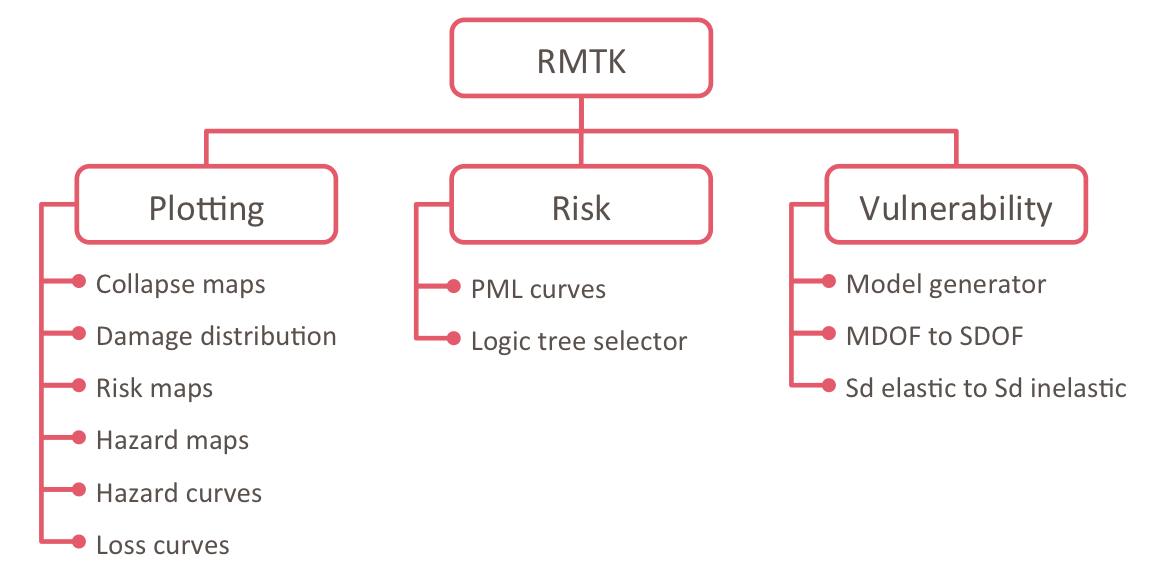
\includegraphics[width=\textwidth]{figures/rmtk_structure.png}
	\caption{The modular structure of the Risk Modeller's Toolkit (RMTK), showing the currently available functionalities}
	\label{fig:rmtk-structure}
\end{figure}